\chapter{Process Design} \label{chapProdProcessDesign}

Process design is a strategic activity aiming at choosing how a production system should behave in production. In particular, all these activities have a strong impact on the inventory level (i.e. the WIP) that, in general, must be kept under control to avoid useless costs, as storage costs, damages costs, cost of searching for materials, cost of the unalignment between physical and information inventory. This chapter focuses on:

\begin{enumerate}
    \item the design of the inventory policy of a production system;
	\item the design of the material handling system;
	\item the design of the workstations.
\end{enumerate}

\section{Inventory policy design (P7)}

Storing goods has a cost. Any supply chain manual, despite its focus, prescribe the \textit{zero inventory} philosophy ~\cite{Womack1992,WomackJ.P.&Jones2000}. Unfortunately, storage levels will never reach zero due to the complexity of the supply chains, their global extensiveness and the fluctuations of the market demand. Hopefully, the right tools can help to set the inventory at an adequate level and to keep it under control. 

\subsection{Model-driven methods (PS4)}
The problem of the inventory design involves the definition of the storage levels for raw materials, semifinished and finished products within the production plant. This problem is addressable by using prescriptive methods which defined the right storage level and the proper rules to replenish the storage (e.g. a re-order point), aiming at reducing storage costs. Storage cost embeds many cost items that are often difficult to estimate. Let assume $h_i=f(q,t)$ be a comprehensive storage cost function, defined as a function of the storage quantity $q$, and the storage time $t$. The problem is to find a policy to minimise the cost $h$, such that:

\begin{itemize}
    \item the inventory level is under statistical control;
    \item the shelflife of items complies with regulations and customers’ expectations;
    \item stockouts are minimised (i.e. the market demand is always satisfied).

\end{itemize}

The type of market demand suggests different prescriptive approaches to the design of the inventory levels. First of all, a key metric to consider is the lead time $LT_i$ necessary to obtain part $i$ from the previous stage of the supply chain (e.g. a supplier or the previous workstation). When $LT_i$ is larger than the amount of time the following node of the supply chain (e.g. a client) is willing to wait, inventory management should be based on predictions. Otherwise, inventory management is deterministic since stock levels can be maintained low by acquiring parts only when needed. Figure \ref{fig_prod_inventory_mgmt} illustrate a model identifying different inventory policies depending on the position of the decoupling point. The decoupling point separates the part of the supply chain where production is organised based on predictions from the part where it is based on the orders. When customers’ willingness to wait is null (e.g. supermarket) or significantly large (e.g. luxury goods as a yacht), the model in Figure \ref{fig_prod_inventory_mgmt} can be stretched on the right (everything is based on the forecasts) or on the left (everything is based on market demand).

% INSERT fig_prod_inventory_mgmt
\begin{figure}[hbt!]
\centering
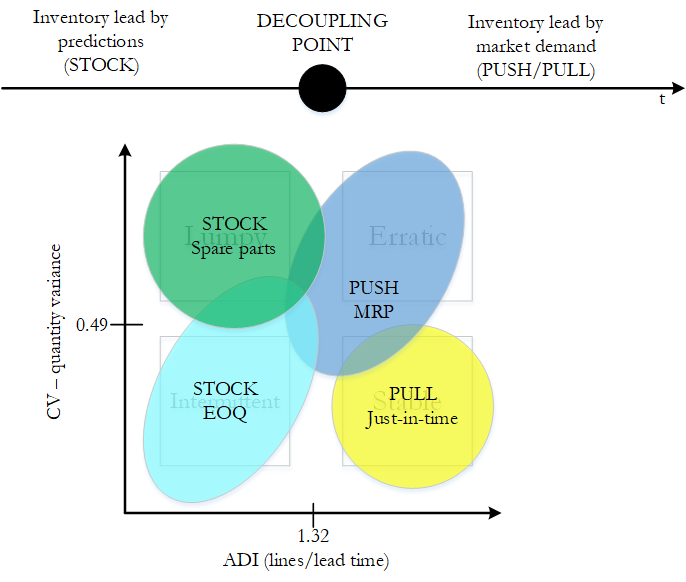
\includegraphics[width=0.9\textwidth]{sectionProduction/design_process_figures/fig_prod_inventory_mgmt.png}
\captionsetup{type=figure}
\caption{Inventory management policies matched with demand patterns.}
\label{fig_prod_inventory_mgmt}
\end{figure}

The demand pattern and the lead time are two typical drivers to choose between stock models and market demand models. There are other drivers as:
\begin{itemize}
    \item the value of the part;
    \item the shared use of the part between many processed (e.g. oil or screws);
    \item the responsiveness and the lead time of the supply chain;
    \item the complexity of the supply chain.

\end{itemize}

In general, stable and erratic parts both have a high frequency of demand. In this case, inventory management can be lead by market demand. The inventory level is defined by making accurate predictions on the market demand (see section \ref{secWorkloadPredictionProd}). These predictions can be used to feed two inventory management paradigms:

\begin{itemize}
    \item the push paradigm;
    \item the pull paradigm (or Just-in-time JIT).

\end{itemize}

On the other side, when predictions are unreliable, the inventory level should be oversized to meet unexpected demand and avoid stockouts. This is the case of:

\begin{itemize}
    \item lot sizing (economic order quantity and safety stock);
    \item spare parts management (e.g. for maintenance reasons).

\end{itemize}

\subsubsection{The push paradigm}
The push paradigm works by pushing finished products into the market. It can be summarised into the statement: \textit{if you can produce a part $i$, then produce $i$}. In other words, when production capacity and raw materials are available, production processes should go on. \par

Under these assumptions, inventory levels should always be enough to feed the production. A standard method to feed production is the Material Requirements Planning (well known as MRP). The MRP identify the order quantities for each part $i$ and for each time period $t$ (time is usually sampled into weeks). This method does not keep the inventory level under control. It only enables the production to satisfy the demand. The method works by considering:

\begin{itemize}
    \item an estimate of the average demand $d_{i,t}$ of part $i$, for each time period $t$;
	\item the quantities of raw materials $\rho$, semifinished $\phi$ and subassemblies $\sigma$ necessary to produce a part $i$;
	\item the production lead time $LT_i$;
	\item the supply lead times $LT_\rho$, $LT_\phi$, $LT_\sigma$;
	\item the current inventory levels $WIP_{i,t}$, $WIP_{\rho,t}$, $WIP_{\phi,t}$, $WIP_{\sigma,t}$.

\end{itemize}

The order quantity for a part $i$ at time $t$ is defined as the difference between the demand $d_{i,t}$ and the inventory level $WIP_{i,t}$. This quantity is, then, corrected to consider the supply and production lead times. Theoretically, the inventory level is out-of-control, but it is kept at a minimum to satisfy the market demand always. In practice, MRP systems are fed with inaccurate predictions and wrong lead times, leading to substantial inventory levels. 

\subsubsection{The pull paradigm}
The pull paradigm has the sole objective of keeping the inventory level under control. The inventory level of a part $i$ is set to:

\begin{equation}
    WIP_i=d_i\times(1+SS)
\end{equation}

Where $SS$ is the percentage of safety stock and $d_i$ is the average market demand. When setting a pull system, it is essential part $i$ has a stable demand pattern; otherwise, $SS$ will be high. $SS$ depends on the ratio between the supply and the production rate of the part. If storage is checked once a day and an additional day is necessary to feed the production, $SS$ should be greater than 2 (given that $d_i$ is expressed parts/days).\par

Usually, a kanban system is used to implement the pull paradigm. A kanban is a label associated with a production order of a given quantity that can be placed within a container with a fixed capacity $q$. The problem is to set the number of kanban for each workstation. This can be calculated as $K=\left\lceil\frac{WIP_i}{q}\right\rceil$.

\subsubsection{Lot sizing \& safety stock}
Lot sizing aims at the definition of the optimal quantity $Q_i$ for an order to run:
\begin{enumerate}
    \item when a re-order point $WIP_i^r$ is reached;
	\item at uniform time intervals (e.g. each week).

\end{enumerate}

Given that this inventory policy makes extensive use of the stock, two costs are considered:

\begin{itemize}
    \item the storage cost;
    \item the cost to send an order.

\end{itemize}

The cost model (EOQ-buy) is defined as follows.

\begin{equation}
    C_i^{BUY}\left(Q\right)=C_i^\prime\left(\frac{Y_i}{Q}\right)+\frac{hQ}{2}
\end{equation}

Where $C_i^{BUY}$ is the cost of setting the size of a lot to $Q$. $C_i^\prime$ is the cost to run an order of part $i$, $Y_i$ is the total expected demand (e.g. parts/year) while $h$ is the storage cost per part. The model assumes a steady demand rate; for this reason, the storage cost is estimated at $\frac{h}{2}$. By setting $\frac{\partial C_i^{BUY}(Q)}{\partial D}=0$, then $Q^\ast=\sqrt{\frac{2C_i^\prime Y}{h}}$.\par

A similar model can be used to set the size of production lot by taking into account:
\begin{itemize}
    \item the storage cost;
    \item the cost of the setup of the machine to process part $i$.

\end{itemize}

The cost model (EOQ-make) is defined as follows.

\begin{equation}
    C_i^{MAKE}\left(Q\right)=C_i^{\prime\prime}\left(\frac{Y_i}{Q}\right)+\frac{hQ\prime}{2}
\end{equation}

Where $C_i^{MAKE}$ is the cost of setting the size of a lot to $Q$. $C_i^\prime$ is the cost of the setup of a workstation to process parts $i$, $Y_i$ is the total expected demand (e.g. parts/year), $h$ is the storage cost per part, $\frac{Q^\prime}{2}$ is an estimate of the average inventory level of parts $i$, and $Q^\prime=Q\left(\frac{X-Y}{X}\right)$, where $X$ is the production quantity. By setting $\frac{\partial C_i^{BUY}(Q)}{\partial D}=0$, then $Q^\ast=\sqrt{\frac{2C_i^{\prime\prime}Y}{h}}\times\sqrt{\frac{X}{X-Y}}$.\par

In general, when the order quantity $Q$ is set, orders can be sent when a re-order point is reached, $WIP_i^r=Y\times LT_i$, where $LT_i$ is the supply lead time for part $i$. Otherwise, in many practical applications, it results simpler to send an order at regular time intervals $RI$ (e.g. every week or every month): $WIP_i^r=Y\times(RI+LT_i)$.\par

In practice, the storage cost of $WIP_i^r$ is lower than the cost of a stockout. For this reason, the storage level $WIP_i^r$ is increased by a safety stock $SS_i$. The level of service (i.e. the probability of having a part $i$ available to serve an order) defines the value of $SS_i$: $Prob\left\{WIP_i^r+SS_i\geq d_i\right\}\geq SL_{i}$.

\subsubsection{Spare parts inventory management}
When dealing with spare parts (lumpy and intermittent parts) the cost minimisation criterion is appropriate as well in the definition of the inventory level for each part. A cost model can be defined by considering the sum of the storage cost and the stockout cost for a part $i$. Let $B_i$ the number of parts required within the time interval considered and $n$ the maximum number of parts that can be stored.

\begin{equation}
\begin{split}
    C_i^\Lambda\left(Q\right)=\\
    h \sum_{q=0}^{Q}q \times Prob\left\{B_i=Q-q\right\} +\\
    + C_md \left(\sum_{q=Q}^{n} Prob\left\{B_i=Q-q\right\} \right)\\
\end{split}
\end{equation}

Where $h$ is the storage cost in $\frac{\euro{} }{part}$, $C_m$ is the cost of the stockout of a part, $d$ is the average absorption rate $\frac{parts}{\tau}$, and $\tau$ is the reference time interval. The $Prob\{Bi=Q-q\}$ indicates the probability of consumption of a number of parts $B_i$ within a time interval $\tau$. An appropriate probability distribution can estimate this value. For example, the Poisson distribution introduced in section \ref{secPoisson}. By setting $\frac{\partial C_i^\Lambda\left(Q\right)}{\partial Q}=0$ the amount of parts $Q$ corresponding to the minimum cost can be found.

\subsection{Data-driven methods}
The definition of the optimal inventory level $Q_i$ of a part $i$ is deeply linked with variables falling out of the control of the production node, as the supply lead time, the demand variability, the service level, the reliability of supply and customers and many other apparently unpredictable variables as global trends, diseases, war and people subjective perceptions. \par

It clearly appears that there is no model able to identify and investigate all these parameters producing a reliable $Q_i$. Big data and the platform economy can help to approach this problem from a different perspective.\par

When supply chain players are willing to share their data using the same logistic platform (see section \ref{secLogPlatform}), the amount of available information is larger, faster and leads to more accurate predictions of the market demand. Under these conditions, the players have robust information at their disposal to set the values of $Q_i$. 

\section{Handling design (P3)}

The handling system allows exchanging material flows between the control points of a production node. The choice of the handling system must be coherent with the chosen inventory policy since it affects the level of WIP of the storage node. Handling systems are characterised using two parameters:

\begin{itemize}
    \item the capacity; i.e. the amount of good that can be transported simultaneously;
    \item the throughput; i.e. the number of goods transported in the unit of time (e.g. parts per hour).
\end{itemize}

The choice of the handling technology is similar to the choice of the processing technology, and the same classification of \ref{secTechChoiceProd} is used. Figure \ref{fig_prod_handling_system} classified handling systems depending on their level of flexibility and automation.

% INSERT fig_prod_handling_system
\begin{figure}[hbt!]
\centering
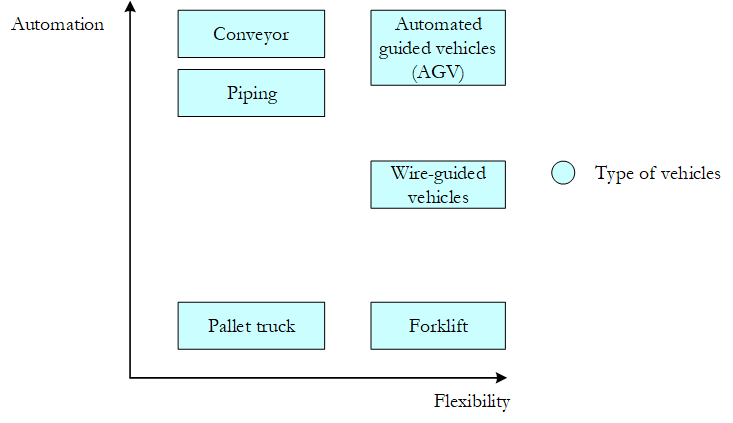
\includegraphics[width=0.9\textwidth]{sectionProduction/design_process_figures/fig_prod_handling_system.png}
\captionsetup{type=figure}
\caption{Flexibility-automation matrix for handling system choice.}
\label{fig_prod_handling_system}
\end{figure}

Figure \ref{fig_prod_handling_system} identifies the most common handling solutions and their position in the classification scheme. The solutions with a high degree of automation help to keep a smooth flow of the production, but they have a fixed throughput that deeply depends on the fleet size or the space available on the plant layout. A conveyor between two working station is a good strategy to fix the amount of WIP to the length of the conveyor; nevertheless, this is possible only if the layout has enough space to hold the conveyor. On the other side, forklift and pallet truck are flexible and adaptable since they only need operators to work. However, their flow is less controllable and more likely to errors and avoidable material flows.

\subsubsection{Model-driven methods (PS3)}
The models to define the handling solution are essentially prescriptive. In many plants, the constraints are so many that the choice of the handling system barely has more than a single alternative.\par

The most common strategy is to define a matrix $F$ with entries assessing the flow of materials $f_{jk}$ exchanged between two workstations $j$, and $k$. Given the graph $G$ with the arcs connecting the workstations, $G$ defines distances $d_{jk}$ with travel time $t_{jk}$. The capacity $C_v$ of a vehicle can be used to define the number of trips ${tr}_{jk}=\left\lceil\frac{f_{jk}}{C_v}\right\rceil\ \left[\frac{trips}{unit\ of\ time}\right]$. The availability of the vehicle a measured in units of times can be used to calculate the minimum fleet size:

\begin{equation}
    N=\frac{{tr}_{jk}\times t_{jk}}{a}
\end{equation}

$N$ is the minimum number since it does not consider all the trips when the vehicle is empty, and it does not consider the dynamics of the system. In addition, it cannot be used for rigid systems as conveyors and pipelines where the dimension of the fleet is represented by the length of the conveyor (the problem is similar to the definition of the optimal inventory level $Q_i$ between workstations $j$, and $k$).\par

For these reasons, discrete events simulation is preferred to assess handling systems from a logistic point of view. All the aforementioned variable are transformed into random variables by considering their probability distribution and the load of the system is simulated instance per instance assessing:

\begin{itemize}
    \item the average saturation of each vehicle, and 
    \item the queues where parts wait to be loaded.

\end{itemize}

This information allows deciding if a solution is suitable from a logistic point of view (i.e. if the throughout of the fleet is appropriate). The final decision must consider multiple alternatives evaluating not only the throughput but also the cost of the handling system. Investment costs are the fixed costs for the equipment. Variable costs usually depend on the level of automation:

\begin{itemize}
    \item both the cost of direct labour and consumables (e.g. the energy) are significant for manual handling systems;
    \item the cost of energy is significant for automated solutions.

\end{itemize}

The logistically feasible solution with the best economic compromise should be chosen as the handling system.

\section{Workstation design (P4)}
The design of the workplace is often considered a minor activity from a supply chain perspective since it is highly peculiar, and guidelines are defined in specific norms which differs depending on the type of work performed. Nevertheless, this stage results relevant from an efficiency perspective since the performance of the operator is enhanced by a well-designed working place.\par

This activity is mainly prescriptive and sometimes related to ergonomics regulations compliance. 

\subsection{Model-driven methods (PS4)}
Here we introduce a method to assess the performance of different workstation setting and support the choice between the alternatives ~\cite{Accorsi2019_cobot}. Two alternatives are usually a business-as-usual (AS-IS) scenario and a TO-BE scenario where the configuration of the workstation changes. The model is valid as well while considering different TO-BE alternatives to be compared. The model identifies three groups of performance indicators:

\begin{itemize}
    \item process parameters, aiming at the evaluation of the efficiency of the workstation;
    \item ergonomic parameters, aiming at the evaluation of the ergonomic workload on the operators of the workstation;
    \item economic parameters, aiming at the evaluation of the fixed and variable costs of the workstation.

\end{itemize}

Figure \ref{fig_prod_workstation_design} identifies these performance parameters. In addition, since many of these choices involves the use of automation of collaborative automation on a workbench, the functional units of the automated scenario are identified. It is important to remember that to perform this type of improvement, together with the economic and technical feasibility, it is necessary to find a high managerial commitment since operators are usually not willing to change the way they are learnt how to work.

% INSERT fig_prod_workstation_design
\begin{figure}[hbt!]
\centering
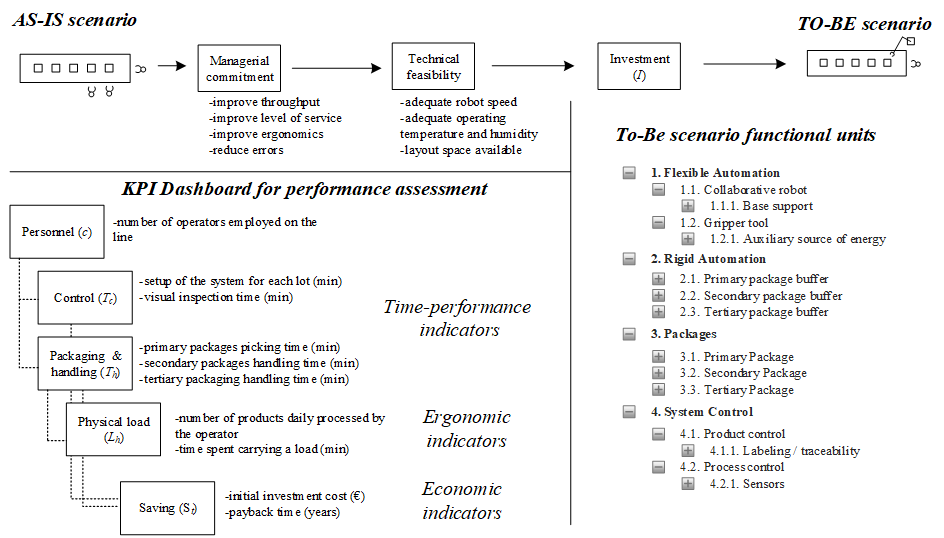
\includegraphics[width=0.9\textwidth]{sectionProduction/design_process_figures/fig_prod_workstation_design.png}
\captionsetup{type=figure}
\caption{A prescriptive model for workbench alternatives comparison.}
\label{fig_prod_workstation_design}
\end{figure}

The main drivers to lead the choice are identified by the performance parameter. If a workstation is able to perform faster, the savings on the hours of direct labour could be enough to support the initial investment. On the other side, when the physical load is significantly reduced, such that:

\begin{itemize}
    \item operators are more precise enhancing the quality of the finished product, or
    \item operators have a lower risk of ergonomic disease.

\end{itemize}

The initial investment may result supported as well. The support and the point of view of the operator are fundamental in this kind of choices to assess whether a workbench configuration results adequate or not.

\section{Applications}

\subsection{Process Design of a food catering plant}
This section analyses the study and redesign of some production and packaging processes in a food catering facility.

\subsubsection{Inventory policy design}
The design of the inventory policy of a food catering facility results deeply linked with the degree of safety f the finished products. While the raw materials storage system follows a rigid first-expiring first-out (FEFO) policy, the problem appears more complex for semifinished and finished products. In particular, a task of the production process becomes critical if attached to a critical control point, according to the HACCP protocol. Since the temperature of a food product must be outside the so-called danger zone (see section \ref{secCateringDesign}), cook-warm products must be kept over 65 \degree C after cooking. All the tasks performed after the cooking area of the plant must be separated by hot-holder working as ovens set to a safe temperature (e.g. 85 \degree C). Figure \ref{fig_prod_CAMST_temperatureProfiles} illustrates the result of a monitoring campaign performed on the temperature of the products leaving the cooking area. Each column identifies a product family while rows identify the tasks performed after cooking.


% INSERT fig_prod_CAMST_temperatureProfiles
\begin{figure}[hbt!]
\centering
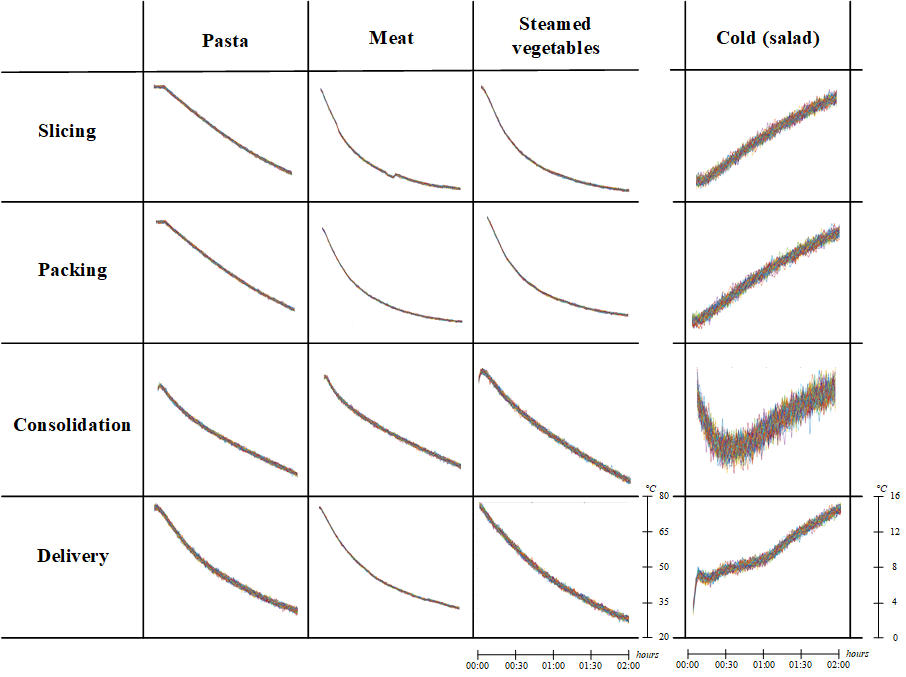
\includegraphics[width=0.9\textwidth]{sectionProduction/design_process_figures/fig_prod_CAMST_temperatureProfiles.png}
\captionsetup{type=figure}
\caption{Temperature decay profiles of products after the cooking department.}
\label{fig_prod_CAMST_temperatureProfiles}
\end{figure}

The number of the hot-holders define their throughput $TH_j$ and the inventory level $Q_i$ between each working station of the end-of-line of a CEKI. By considering the average processing time for each task, it was possible to estimate the temperature decay and to simulate the effect on different production lot. The output of the simulation identifies the adequate number of hot-holder between workstations and between the consolidation area and the shipping bays (for finished products). A minor investment in hot-holding machine and additional space for the plant layout reduced the errors and increased the quality of the finished product ~\cite{Tufano2020}.

\subsubsection{Handling design}
The design of the handling of a CEKI is static and relies on the high flexibility of manual handling using roll containers. Roll dimensions compatible with blast-chiller and ovens and entire lots can be cooked or refrigerated without additional handling. In addition, the low throughput of the plant does not identify the need for automation of the handling systems.

\subsubsection{Workstation design}
The activity on a packing workstation of a CEKI is highly repetitive with many identical moves that may lead to errors (e.g. a product placed in the wrong pack) when the operator is tired. For this reason, the technical and economic feasibility of the implementation of automated collaborative technology in manual handling/production processes is studied ~\cite{Accorsi2019_cobot}. The technical and economic assessment evaluate the placement of a cobot replacing the human operator in charge of loading the plastic boxes containing the finished products.\par

The cobot has a kinematic that can be easily programmed and simulated; for this reason, it is fast to extrapolate the expectation of the operative time and motions (these values have the superscript $\alpha$). These values have to be compared with the human performance that is measured on-field in the business-as-usual scenario (marked by the superscript $\beta$). The saving per year is calculated as:

\begin{equation}
    S_t=\left(\left(t^{idle}+t_{pick}^\alpha\right)\times l^\alpha+\left(t_{pick}^\beta+t_{depot}^\beta\right)\times\left\lceil\frac{l^\alpha}{v^{\alpha,\beta}}\right\rceil-t^{trav}\right)\times l\times d\times c-c^{maint}
\end{equation}

Where: $t^{idle}$ is the idle time of the operator waiting for packed meals at the end-of-line (sec); $t_{pick}^\alpha$ is the time to label a primary package (sec); $l^\alpha$ is the number of primary packages per production lot; $t_{pick}^\beta$ is the time to pick an empty secondary package and put it into a filling buffer (sec); $t_{depot}^\beta$ time to put a full secondary package into a tertiary package (sec); $v^{\alpha,\beta}$ is the number of primary packages per secondary package; $t^{trav}$ is the travelling time to supervise production tasks (sec); $l$ is the number of lots per working shift; $d$ is the number of working shifts per year; $c$ is the cost of an operator for a working shift (\euro{}); $c^{maint}$ is the maintenance cost of the cobot per year. \par

Since the value of $S_t$ increases rapidly year by year, the investment in automation resulted convenient for the company.

%\clearpage
\bibliographystyle{ieeetr}
\bibliography{sectionProduction/design_process_ref}
	
